%%% Compile using: pdflatex main.tex %%%
\documentclass[a4paper,12pt]{article}
\usepackage{mypackages}

\title{\textbf{MNXB01} - Project report}
\date{\today}
\author{Cameron Robertson, \and Viktor Drugge, \and Louise Villander}

\begin{document}
	\maketitle
	\section{Introduction}
	\label{sec:pre}
	In this report, urban adjusted temperatures from the Uppsala data center will be analysed
	and graphed, with a particular focus on Spring temperatures. Samples of temperatures during certain
	days will also be plotted. Finally, the data will be used to determine the beginning of Spring, through
	the temperature definition. To do this, ROOT version 5.34/30 is used.
	\documentclass[a4paper,10pt,oneside]{article}

%\usepackage{ucs}
\usepackage[utf8]{inputenc}
%\usepackage{babel}
%\usepackage{fontenc}
\usepackage[pdftex]{graphicx}

\usepackage[dvips,pdftex]{hyperref}

\author{Cameron Robertson}
\date{11/09/17}

\begin{document}

\section{Introduction}
\label{sec:intro}

 In this section, the temperature
data from Uppsala will be analysed with the aid of histograms, which show the mean daily
temperatures from 1722 until 2013. Each histogram will show data for a specific day of the year,
so it may be enlightening to look at all 366 potential histograms, though this would
not be practical. Instead, a few specific dates will be chosen to analyse the histogram
distribution. It will then be determined how useful these results will be in determining the beginning
of Spring.

\section{Extracting the data}
\label{sec:data}

The Uppsala temperature data was given as a space seperated list, with the first three
columns representing the year, month and day respectively. The fourth column included the mean
temperature of that day unadjusted for urban effect, whereas the fifth column held
the same, but adjusted for urban effect. The temperatures to be plotted were those 
in the fifth column. The sixth held an id number to represent the weather station
that the temperature was recorded from. For the purposes of this project, only Uppsala
data was needed, which had an id of 1.

The function to extract the required information took two arguments: a day and a month. Firstly, each column was streamed into a vector. This was
easier and safer than using an array, since vectors dynamically change size. A for loop was then run which streamed the appropriate vector elements for the
chosen month and day into another file. This also only streamed the data with an id of 1. The data in the file was then streamed back into another
vector, which was then used to plot the histogram

\section{Results and Discussion}
\label{sec:res}

\begin{figure} 
  \begin{center}
    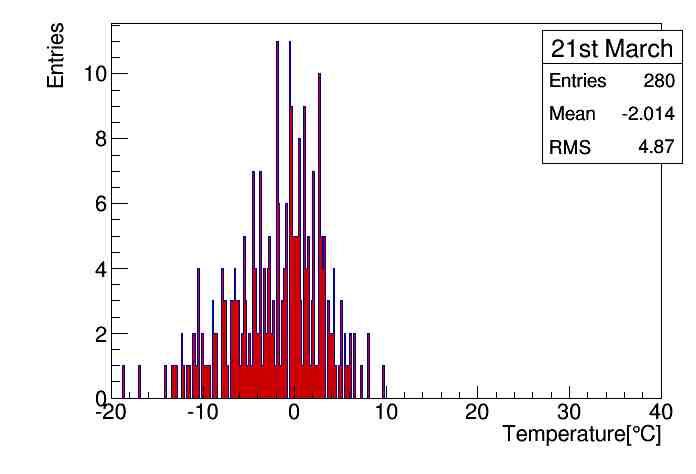
\includegraphics[width=10cm]{/home/courseuser/Project/Project/Code/Equinox_temps.jpg}
    \caption{Histogram showing temperatures from 1722-2013 at 21.3}
    \label{fig:vern}
  \end{center}
\end{figure}

Clearly \ref{fig:vern} shows that very generally, the temperature in Uppsala at the
vernal equinox tends to be below 0 degrees, which is colder than previously expected, especially given the previous
results from this report. However, the rather high standard deviation
shown in \ref{fig:vern} displays just how much variation in temperature there is over 300 years.
The range is also expectedly quite large, owing to the large quantity of data. Also, there have been several cases of extremely
cold temperatures, which could have altered the mean.

\begin{figure}
 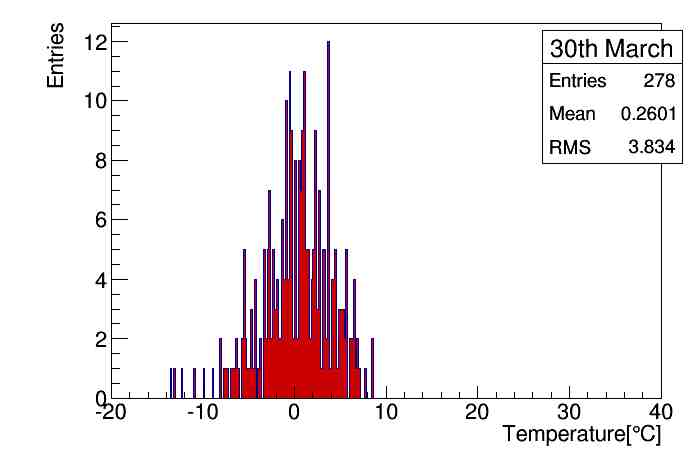
\includegraphics[width=10cm]{/home/courseuser/Project/Project/Code/week.jpg}
 \caption{Histogram showing temperatures from 1722-2013 at 30.3}
 \label{fig:week}
\end{figure}

Comparing \ref{fig:week} to \ref{fig:vern}, the mean temperature has clearly increased significantly even
after just one week, with the mean temperature now being above freezing. Notably, the standard deviation
has also decreased slightly, so the spread of results for this day is slightly lower than on the previous histogram, though is
still quite high.

\begin{figure}
 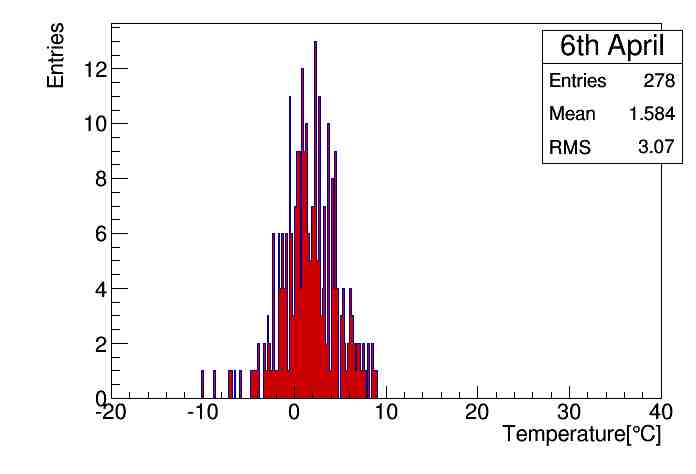
\includegraphics[width=10cm]{/home/courseuser/Project/Project/Code/2week.jpg}
 \caption{Histogram showing temperatures from 1722-2013 at 6.3}
 \label{fig:twoweek}
\end{figure}

The same trend continues one week on from this, as shown by \ref{fig:twoweek}. The mean temperature has again increased significantly
, though by a smaller value this time. Most notably, the spread of data has decreased, resulting in a visibly thinner histogram, resulting
in a lower standard deviation.

\section{Conclusion}
\label{sec:conc}

The results show that the large amount of data nevertheless still shows the expected trend of increasing temperature from week
to week, despite large standard deviation and recurring data from very cold years, which can be seen on
the left side of all the histograms. Theoretically, it would be possible to find the mean warmest and coldest day between 1722-2013,
but this would require repeatedly running the aforementioned function until the minimum and maximum values were found
It would also be difficult to determine the beginning of Spring(Using the temperature definition) using this program,
as a similar brute force method would be required, and it would be difficult to plot the results.






 
\end{document}

	\documentclass[a4paper,12pt]{article}
\usepackage{mypackages}

\begin{document}
\section{Calculating the start of spring}
In order to properly calculate at which date spring starts, a 
definition for the season is necessary. On the webpage of SMHI 
(\url{https://www.smhi.se/kunskapsbanken/meteorologi/var-1.1080})
a meteorological definition of spring is given. Below is the 
definition of the start of spring from SMHI.

\hfill\begin{minipage}[c]{\textwidth-2cm}
	If the daily average temperature is above 0 $^\circ$C but below 10 
	$^\circ$C, we call this for a day with spring temperature. If this 
	occurs seven days in a row,	we say that spring arrived the first of 
	these days. Even if there is a return to lower temperatures then it is
	still counting as spring.
	\newline
	$\ldots$
	\newline
	The start of spring can not occur before the 15th of febuary.
	\newline
	$\ldots$
	\newline
	Spring can, at latest, occur the 31th of July.
\end{minipage}

\noindent Using this definition, the temperature for spring arrival was 
extracted from the data. The method for reading, extracting, plotting, 
and, fitting the data is performed in a single method. There exist 
several ways to implement a solution of the posed question of spring 
arrival. The choice of using a single method is one of them. The inital 
set of lines of "springArrive()" initialize variables that will be used 
when reading the data file "uppsala\_tm\_1722-2013.dat".
\\\indent
The exact date for when each season start and end are not fixt and may 
vary a lot between each year. Using only the first paragraph of the 
above definition dates as late as november could be classified as the 
beginning of spring. For this reason, we use the last of July as a 
cutoff point. The beginning of spring may change a lot depending on 
location. The definition used here was found most promising for the 
data set of Uppsala. 

The main part of the springArrive() method occur in the while loop. It 
can be summarized in two parts. First check if the spring of the 
current year is found using the foundSpring variable. If foundSpring is 
true, the current year is extracted and the file pointer is moved down 
the file till it finds the next year. Note that when this loop is 
complete the the next line read will represent the earliest date
of next year given in the data file.

\begin{lstlisting}
if(foundSpring == true)
	{
		dayCount = 0;
		foundSpring = false;
		Int_t nextYear = year+1;
		while(nextYear != year)
		{
			if(getline(file,line, '\n'))
			{
				stringstream ssNextYear(line);
				ssNextYear >> year >> month >> day >> temp >> temp_urban >> id; 
			}
			else
				break;
		}
	}
\end{lstlisting}
If foundSpring is false, the file pointer is pointing at a year which 
has not yet been registered. In this case the second loop is used. 
Here, the program try performing a for loop representing the 7 day span 
required by the definition above. The id of the data is checked with 
the provided "dataset" variable so to  ensure only data from the 
correct data set is stored. Next, the temperature is examined, it has 
to be between 0 $^\circ$C and 10$^\circ$C. dayCount represent the 
total number of dates iterated of the year, regardless of id number. 
This ensures that spring will be identified even if data points might 
be missing. As a final requirement, the month can not exceed July, in 
line with the definition of SMHI. At the final iteration of the for 
loop, the first registered date and temperature is stored. Note the 
method does not divide the year into 52 weeks but instead look for the 
first 7 succeeding iterations which satisfy the definition we use.
\begin{lstlisting}
if(foundSpring == false)
	for(Int_t i=0; i < daysWeek; i++)
		{
			Double_t tmp;
			getline(file,line, '\n');
			stringstream ss(line);
			if(ss >> year >> month >> day >> temp >> temp_urban >> id) //check output can is eligible
			{
				dayCount++;
				if(id==dataset)//Take data from dataset
				{
					//dayCount>=46 represent 15 feb (minimum date for spring), month<8 
					remove missing data (otherwise autumn is classified as spring)
					if(temp_urban >= 0 && temp_urban <= 10 && dayCount >= 46 && month 
					< 8) //Check if temperature fulfill definition of spring
					{
						if(i==0)
						{
							sYear=year; sMonth=month; sDay=day;
							sTemp=temp_urban;
						}
						if(i == daysWeek-1) //Save temp of first day
						{
							foundSpring = true;
							hDays->Fill(dayCount - (daysWeek+1)); //(daysWeek+1), 
							+1 because dayCount incremented by 1 previously
							hTemp->Fill(sTemp);
							//Print date of spring
							cout << "Spring found:\t" << sYear << "\t" << sMonth << "\t" << sDay << "\t" << sTemp << endl;
							springDate << sYear << "\t" << sMonth << "\t" << sDay << "\t-\t" << sTemp << endl;
						}
					}
					else //If temperature is not in interval, start new iteration
						break;
				}
			}
		}
\end{lstlisting}
The date of each spring found is stored in a file 
"found\_spring\_date.dat". The registered days are saved in a histogram 
that span one year. The resulting histogram can be seen in figure 
\ref{fig:SA_dayHist}. Note the sharp start at day 46, representing the 
15th of february. The mean of the histogram, day 80, represent the 21 
of March if its not a leap year and the 20 of March otherwise. A total 
of 365 bins are used. One for each day, as seen on the x-axis, and, the 
y-axis represent the number of entries. For each date registered, the 
temperature is saved in a histogram, see figure \ref{fig:SA_tempHist} 
for more details. Here, the x-axis represent the temperature interval 
and the y-axis the number of entries. The resulting histogram is fitted 
to a exponential function,
\begin{equation}
	f(x)=\alpha e^{-\lambda x}.\label{eq:SA_fitfunc}
\end{equation}
The curve fit relatively well with the histogram. This is expected as 
the gradual increase of the temperature each spring should result in 
the majority of temperatures ending up in the low temperature region.
\begin{figure}[htb]
	\centering
	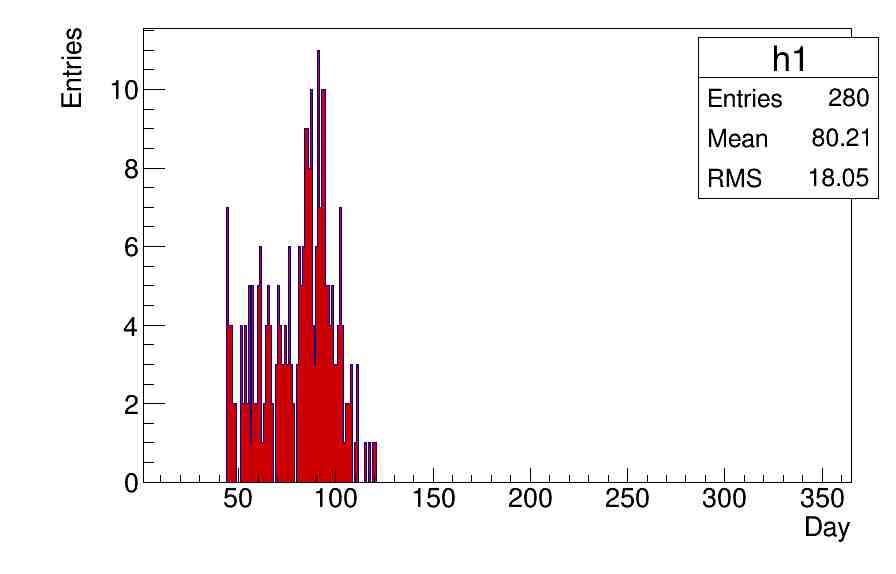
\includegraphics[scale=.4]{../Code/springArrive_dayHist.jpg}
	\caption{Number of times spring has arrived since the 18th century 
	in Uppsala using the meteorological definition of SMHI. Day 80, the 
	mean of this histogram, represent either March 20 if its a leap year 
	or March 21 if its not a leap year. Note the sharp peak at day 46, 
	representing the 15th of febuary. Dates after the last of July are not 
	included. The histogram consist of 365 bins, one for each day of the 
	year, seen on the x-axis, and, the number of entries on the y-axis. 
	This binning shifts leap years by one day, however the effect is 
	neglectable.}
	\label{fig:SA_dayHist}
\end{figure}
\begin{figure}[htb]
	\centering
	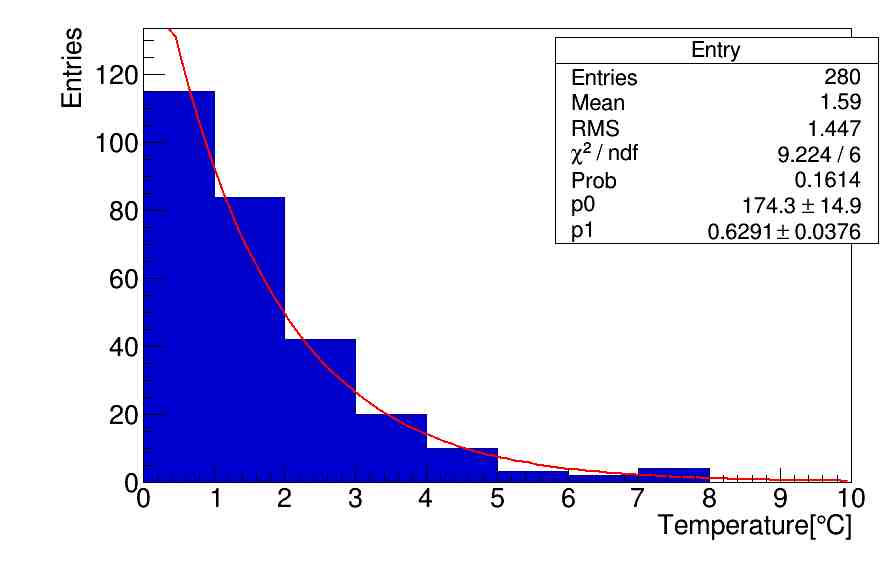
\includegraphics[scale=.4]{../Code/springArrive_tempHist.jpg}
	\caption{Temperature histogram for all spring arrival dates (blue) and 
	fitted exponential function (red line), see equation 
	\eqref{eq:SA_fitfunc}. The histogram fit relatively well with a 
	exponential function, as expected since the gradual increase of the 
	temperature each year should yield a decaying distribution. Here, 
	$p0$ represent $\alpha$, and, $p1$ represent $\lambda$ of equation 
	\eqref{eq:SA_fitfunc}. The x-axis represent the temperature in 
	$^\circ$C and the y-axis the number of entries.}
	\label{fig:SA_tempHist}
\end{figure}

\end{document}

	\documentclass[a4paper,12pt,twoside]{article}
\usepackage{mypackage}

\begin{document}
 \section{Calculating the mean temperatures of every day of the year}
 \label{sec:3.2}
 How does the temperature change over the course of a year? Recording the temperature
 every day for one year might give some indication, but leaves a large margin of error.
 With a dataset stretching almost three hundred years we can calculate the mean
 temperature of each day and get a much more reliable result.
 
 The mean temperature of a certain day is the sum of the temperatures recorded at
 that day, divided by the number of days it has been recorded:
 \begin{equation}
  \label{eq:MeanTempPerDay}
  \overline{T(day 1)} = \frac{T(day 1, year 1)+T(day 1, year 2)+...+T(day 1, year N)}{N}
 \end{equation} 
  
 
 Reading from the datafile, each datatype was put in a vector (excluding the year
 1722 since we don't have all the data for that year, and the 29th of february for
 simplicity). We now have the data in vectors of equal length $(2013-1722)\times(365)=106215$,
 where the data in the same position in the vectors correlate.
 
 Next, the data needed to be separated according to which year it belonged. An empty
 vector of length 365 was created, and then (using a for-loop) the temperature belonging
 to day $k$ was added to the $(k-1)$:th position in the vector. The number of times this
 summation happened was also recorded (it should be equal to the number of years, $291$).
 
 \begin{verbatim}
  	//loop for calculating the mean temperatures of each day
	for (UInt_t k=0; k < vyear.size(); k++){
	
	...
	
	if (vyear.at(k) != vyear.at(k+1)){
		daycounter = 365;
	  }

	else if (vyear.at(k) == vyear.at(k+1)){
	  daycounter = daycounter+1;
	  }
	
	sumtempvec.at(daycounter-1)
	          =sumtempvec.at(daycounter-1) + vtemp.at(k);
	
	...
	
	if (daycounter == 365){
	  daycounter = 0;
	  yr_it = yr_it +1; //the number of years we've iterated over
	  }
	}
 \end{verbatim}
 Using another for-loop to divide each element of the vector with the number of years,
 we now had a vector where each element was the mean temperature of the day
 corresponding to the element's position.
 \newline
 The standard deviation is defined as 
  \begin{equation}
 \label{eq:StdDev}
 \sigma = \sqrt{\frac{\sum\limits_{i=1}^{n} (t_{i}-\bar{t})^2}{n-1}}
 \end{equation}
 
 The mean temperature of each day $\bar{t}$ had been calculated as above, and now another 
 empty vector of length 365 was created. In the same way as before, we looped over the vectors
 containing the data, this time putting the square of the sum of the differences between the
 temperature of the current iteration and the mean temperature of the current day in the vector:
 
 \begin{verbatim}
    	...
  	vStdDev.at(daycounter-1) +=
  	    (vtemp.at(k)-sumtempvec.at(daycounter-1))*
  	    (vtemp.at(k)-sumtempvec.at(daycounter-1));
  	...
 \end{verbatim}

 
 After the iteration we therefore had ${\sum\limits_{i=1}^{n} (t_i - \bar{t})}^2$. Using another for-loop, each element in the vector
 was then divided by the number of years ($n$) in the same way as before and the square root of these values was
 calculated, to get the standard deviation for each day of the year.
 
 \begin{verbatim}
	for (UInt_t q=0;q<vStdDev.size();q++){
	  vStdDev.at(q) = TMath::Sqrt(vStdDev.at(q)/(yr_it-1));
	}
 \end{verbatim}
 
 Finally we had two vectos, one containing the mean temperatures of each day, and the other
 containing the standard deviation, where the position in the vector correlated to the day
 of a year. Using yet another for-loop, the elements in the two vectors were set to be the
 bin content and the bin errors in a histogram. This produced the histogram shown in
 figure \ref{fig:tempPerDay}.
 
 \begin{figure}[htb]
  \begin{center}
   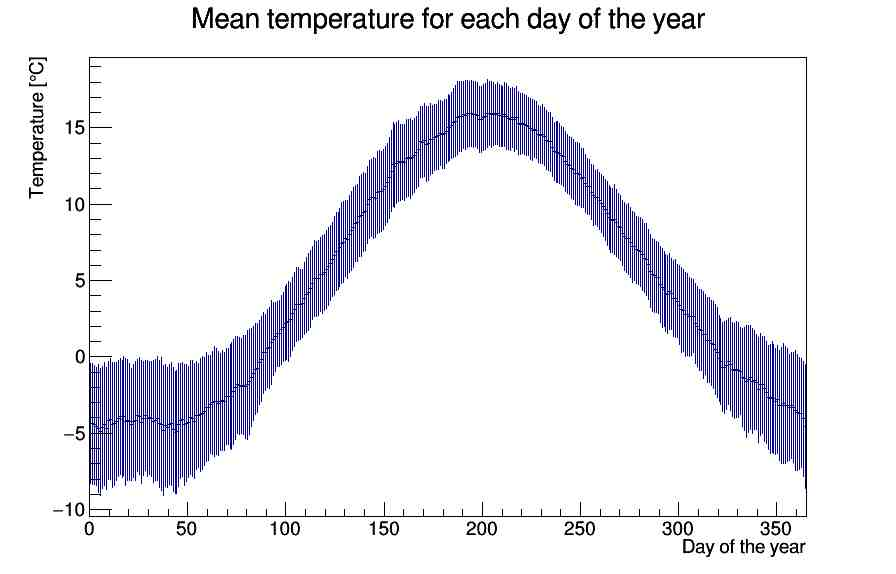
\includegraphics[width=13cm]{../Code/tempPerDay.jpg}
   \caption{Histogram showing the mean temperature of every day of the year}
   \label{fig:tempPerDay}
  \end{center}
 \end{figure}
 
 From the histogram we can see that the temperature is at its peak around day 200, that is July 19, and
 not surprisingly it is coldest around New Years and the beginning of the year. The mean temperature remains
 approximately constant at around $-4 ^{\circ}$C until day 50 (February 19), when it begins to rise and crosses into
 positive temperatures around day 95 (April 5). However, the error bars showing deviations from the mean allow for a large
 variation of temperature of approximately $15 ^{\circ}$C in the beginning of the year (this decreases to approximately $5 ^{\circ}$C
 later on), showing that the temperatures during springtime can vary greatly from year to year.
 
 
\end{document}




	
	\section{Conclusion}
	\label{sec:con}
	This report has demonstrated some of the results from analysis of the Uppsala dataset. Despite the sporadic nature of temperature when 
	taken over a long period of time, we have seen that viable conclusions and results can be derived. The mean temperature of a given day was seen to be quite variable depending on 
	which day was inputted, but the general trend over a number of days was as expected (increase throughout late March). Interestingly, extracting the spring date of each year
	suggested March 20th or March 21th as the average date of spring arrival, in line with the commonly accepted date. Plotting the temperature of all determined dates resulted in a 
	histogram that fitted well with a exponential function, this is as expected since on average the temperature increase gradually each spring. Leap years shift dates after the 28th
	of february which affect the results, but this is of minor concern since the standard deviation is relatively high, even when shifting the dates by one day. Plotting the mean temperatures
	of every day shows how much temperatures vary over the course of a year, and also that temperatures can vary quite a lot from year to year on the same date, particularly during the end 
	of winter and in spring.
\end{document}
